%%%%%%%%%%%%%%%%%%%%%%%%%%%%%%%%%%%%%%%%%%%%%%%%%%%%%%%%%%%%%%%%%%%%%%%%%%%%%%%%%%%%%%%%%%%%%%%%%%%%%%%
%%%%%%%%%%%%%% Template de Artigo Adaptado para Trabalho de Conclusão de Curso - SI Contagem - PUCMINAS %%%%%%%%%%%%%%%%%%%%%%%%
%% codificação UTF-8 - Abntex - Latex -  							     %%
%% Autor da primeira versão:    Fábio Leandro Rodrigues Cordeiro  (fabioleandro@pucminas.br)                            %% 
%% Co-autor da primeira versão: Prof. João Paulo Domingos Silva, Harison da Silva e Anderson Carvalho                   %%
%% Revisores normas NBR (Padrão PUC Minas) da primeira versão: Helenice Rego Cunha e Prof. Theldo Cruz                  %%
%% Versão: 1.1     18 de dezembro 2015                     	                                     %%
%%%%%%%%%%%%%%%%%%%%%%%%%%%%%%%%%%%%%%%%%%%%%%%%%%%%%%%%%%%%%%%%%%%%%%%%%%%%%%%%%%%%%%%%%%%%%%%%%%%%%%%


\documentclass[a4paper,12pt]{article}
\usepackage{times}
\usepackage{abakos}  %pacote com padrão da Abakos baseado no padrão da PUC
%%%%%%%%%%%%%%%%%%%%%%%%%%%
%Capa da revista
%%%%%%%%%%%%%%%%%%%%%%%%%%

%\setcounter{page}{80} %iniciar contador de pagina de valor especificado
\newcommand{\monog}{Dispositivos de Lógica Programável aplicado em automação industrial
}
%\newcommand{\monogES}{Article template Institute of Mathematical Sciences and Informatics}
\newcommand{\tipo}{Artigo}  % Especificar a seção tipo do trabalho: Artigo, Resumo, Tese, Dociê etc
\newcommand{\origem}{Brasil}
%\newcommand{\editorial}{Belo Horizonte, p. 01-11, nov. 2024}  % p. xx-xx – páginas inicial-final do artigo
\newcommand{\editorial}{}  
\newcommand{\lcc}{\scriptsize{Licença Creative Commons Attribution-NonCommercial-NoDerivs 3.0 Unported}}

%%%%%%%%%%%%%%%%%INFORMAÇÕES SOBRE AUTOR PRINCIPAL %%%%%%%%%%%%%%%%%%%%%%%%%%%%%%%
\newcommand{\AutorA}{Davi Cândido de Almeida}
\newcommand{\funcaoA}{}
\newcommand{\emailA}{\href{Davi Cândido de Almeida: 104103@sga.pucminas.br}{1527368@sga.pucminas.br}}
\newcommand{\cursA}{Aluno(a) do Programa de Graduação em Ciência da Computação}

\newcommand{\AutorB}{Theldo Cruz Franqueira}
\newcommand{\funcaoB}{}
\newcommand{\emailB}{\href{Theldo Cruz Franqueira: 104103@sga.pucminas.br}{104103@sga.pucminas.br}}
\newcommand{\cursB}{Professor(a) do Programa de Graduação em Ciência da Computação}
% 
% Definir macros para o nome da Instituição, da Faculdade, etc.
\newcommand{\univ}{Pontifícia Universidade Católica de Minas Gerais}

\newcommand{\keyword}[1]{\textsf{#1}}

%Para as URLS não ultrapassarem a margem
\usepackage{url}
\makeatletter
\g@addto@macro{\UrlBreaks}{\UrlOrds}
\makeatother

\usepackage{adjustbox} % reduzir tamanho figuras

\usetikzlibrary{arrows,shapes,positioning,shadows,trees}

\tikzset{
  basic/.style  = {draw, text width=3cm, drop shadow, font=\sffamily, rectangle},
  root/.style   = {basic, rounded corners=2pt, thin, align=center,
                   fill=blue!30},
  level 2/.style = {basic, rounded corners=6pt, thin,align=center, fill=green!30,
                   text width=8em},
  level 3/.style = {basic, thin, align=left, fill=pink!60, text width=6.5em}
}

\begin{document}
% %%%%%%%%%%%%%%%%%%%%%%%%%%%%%%%%%%
% %% Pagina de titulo
% %%%%%%%%%%%%%%%%%%%%%%%%%%%%%%%%%%

\begin{center}

\includegraphics[scale=0.2]{figuras/brasao.jpg} \\
PONTIFÍCIA UNIVERSIDADE CATÓLICA DE MINAS GERAIS \\
Instituto de Ciências Exatas e de Informática

% \vspace{1.0cm}

\end{center}

 \vspace{0cm} {
 \singlespacing \Large{\monog \symbolfootnote[1]{Artigo apresentado ao Instituto de Ciências Exatas e Informática da Pontifícia Universidade Católica de \linebreak Minas Gerais, campus Coração Eucaristico, como pré-requisito parcial para obtenção do título de Bacharel em Ciência da computação.} \\ }
 % \normalsize{\monogES}
 }

\vspace{1.0cm}

\begin{flushright}
\singlespacing 
\normalsize{\AutorA \footnote{\funcaoA \cursA \,-- \emailA . }} \\
\normalsize{\AutorB \footnote{\funcaoB \cursB \,-- \emailB . }} \\
%\normalsize{\AutorC \footnote{\funcaoC \cursC \,-- \emailC . }} \\
%\normalsize{\AutorD \footnote{\funcaD \cursD \,-- \emailD . }} \\
\end{flushright}
\thispagestyle{empty}

\vspace{1.0cm}

\begin{abstract}
\noindent
O presente artigo explora a utilização de Dispositivos Lógicos Programáveis Complexos (CPLDs) na automação industrial, destacando seu papel na otimização de processos e na redução de custos de produção. Com o crescente avanço das tecnologias eletrônicas, os CPLDs surgem como uma alternativa versátil aos Controladores Lógicos Programáveis tradicionais, oferecendo interfaces amigáveis e a capacidade de reconfiguração. O estudos analisados se propõe a analisar e descrever conceitos da literatura acadêmica sobre CPLDs, visando entender suas aplicações industriais, benefícios e terminologias associadas. O artigo aborda a evolução dos circuitos digitais, destacando a importância de tecnologias como ASICs, ASSPs e FPGAs, PROMs, PLAs e PALs. Os CPLDs são apresentados como uma solução flexível e eficiente, capaz de atender às necessidades de inovação tecnológica em diversos setores, permitindo a adaptação rápida a novas demandas. Assim, o presente trabalho busca a construção de uma base sólida de conhecimento sobre o funcionamento e as aplicações dos CPLDs, ressaltando sua relevância na automação industrial moderna.
\\\textbf{\keyword{Palavras-chave:}} CPLDs; FPGA; PROM; PLA; PAL.
\end{abstract}

\vspace{3.0cm}

%%%%%%%%%%%%%%%%%%%%%%%%%%%%%%%%%%%%%%%%%%%%%%%%%%%%%%%%%
\selectlanguage{english}
\begin{abstract}
\noindent
The present article explores the use of Complex Programmable Logic Devices (CPLDs) in industrial automation, highlighting their role in process optimization and production cost reduction. With the ongoing advancement of electronic technologies, CPLDs emerge as a versatile alternative to traditional Programmable Logic Controllers, offering user-friendly interfaces and reconfigurability. The studies reviewed aim to analyze and describe academic literature on CPLDs, with the goal of understanding their industrial applications, benefits, and associated terminologies. The article discusses the evolution of digital circuits, emphasizing the importance of technologies such as ASICs, ASSPs, FPGAs, PROMs, PLAs, and PALs. CPLDs are presented as a flexible and efficient solution capable of meeting technological innovation needs across various sectors, allowing for quick adaptation to new demands. Thus, this work seeks to build a solid foundation of knowledge on the functionality and applications of CPLDs, highlighting their relevance in modern industrial automation.
\\\textbf{\keyword{Palavras-chave:}} CPLDs; FPGA; PROM; PLA; PAL.
\end{abstract}

\selectlanguage{brazilian}
 \onehalfspace  % espaçamento 1.5 entre linhas
 \setlength{\parindent}{1.25cm}

%%%%%%%%%%%%%%%%%%%%%%%%%%%%%%%%%%%%%%%%%%%%%%%%%
%% INICIO DO TEXTO
%%%%%%%%%%%%%%%%%%%%%%%%%%%%%%%%%%%%%%%%%%%%%%%%%

%%%%%%%%%%%%%%%%%%%%%%%%%%%%%%%%%%%%%%%%%%%%%%%%%%%%%%%%%%%%%%%%%%%%%%%%%%%%%%%%%%%%%%%%%%%%%%%%%%%%%%%%%%%%%%%%%%%%%%%%%%%%%%%%
%%%%%%%%%%%%%% Template de Artigo Adaptado para Trabalho de Conclusão de Curso - SI Contagem - PUCMINAS                       %%
%% codificação UTF-8 - Abntex - Latex -  							                                                          %%
%% Autor da primeira versão:    Fábio Leandro Rodrigues Cordeiro                                                              %% 
%% Co-autores da primeira versão: Prof. João Paulo Domingos Silva, Harison da Silva e Anderson Carvalho		                  %%
%% Revisores normas NBR (Padrão PUC Minas) da primeira versão: Helenice Rego Cunha e Prof. Theldo Cruz                        %%
%% Versão: 1.1     18 de dezembro 2015                                                                                        %%
%%%%%%%%%%%%%%%%%%%%%%%%%%%%%%%%%%%%%%%%%%%%%%%%%%%%%%%%%%%%%%%%%%%%%%%%%%%%%%%%%%%%%%%%%%%%%%%%%%%%%%%%%%%%%%%%%%%%%%%%%%%%%%%%
\section{\esp Introdução} 

Indústrias de diversos segmentos buscam constantemente a redução de custos de produção, bem como alternativas para facilitar o gerenciamento e otimizar seus processos. Portanto, o desenvolvimento de novas tecnologias alternativas se apresenta como uma chance da redução e otimização de todo o seu processo logístico. Em meio a isso, os CLPS (Dispositivos de lógica Programável Complexa) se apresentam como uma alternativa promissora para além de reduzir custos, também facilitar a sua própria utilização, a partir de interfaces mais amigáveis e o uso de linguagens modernas, sendo a alta durabilidade e versatilidade qualidades também alcançada por estes dispositivos em comparação com os clássicos Controlador lógico Programável ou CLP
\cite{Freitas2015}

\begin{citacaodireta}
A crescente evolução do mercado de circuitos eletrônicos é visível. Um exemplo para esta afirmação é o mercado mundial, influenciado drasticamente pela produção de componentes eletrônicos. Porém, muitos autores citam que a verdadeira virada no mercado eletrônico do século XX foi a criação dos circuitos de aplicação específica e o aperfeiçoamento do hardware reconfigurável dos Dispositivos Lógicos Programáveis (Programmable Logic Device - PLD) 
\cite[25]{Oliveira2011}.
\end{citacaodireta}

Tratando-se de uma tecnologia nova sua utilização abre portas para o desenvolvimento de novas aplicações em automação industrial, no qual será explorado e analisado neste artigo, e com isso buscar a construção de uma base sólida de entendimento sobre seu funcionamento e aplicações.

\section{\esp Objetivo}

Analisar artigos e produções acadêmicas sobre CLPDs, buscando contribuir para o entendimento de suas aplicações industriais, bem como de seus benefícios e terminologias envolvidas, visando construir uma base sólida de conhecimento através da mescla dos recentes conhecimentos obtidos através de estudos em arquitetura de computadores, como circuitos lógicos combinacionais e sequenciais, com o entendimento de suas aplicações na indústria.

\subsection{\esp Justificativa} 
\label{subsec:1}
As tecnologias envolvidas em dispositivos CPLD (Complex Programmable Logic Devices) abrangem amplamente conceitos de circuitos e portas lógicas, fundamentais em áreas como informática e equipamentos industriais. Elas também se integram a noções trabalhadas nas disciplinas de arquitetura de computadores, com foco na reconfiguração de hardware e otimização de custos lógicos e processuais. Portanto, por ser um dispositivo lógico programável que prioriza a redução das relações custo-benefício, seu estudo se apresenta como uma oportunidade valiosa para compreender e explorar soluções de hardware que oferecem flexibilidade, eficiência e escalabilidade. Além disso, o CPLD permite o desenvolvimento de sistemas que podem ser rapidamente adaptados a novas necessidades, tornando-se uma ferramenta essencial para a inovação tecnológica em diversos setores.

\section{\esp Tecnologias dos Dispositivos Lógicos Programáveis}

\subsection{\esp Os Circuitos Digitais  }
Durante as últimas décadas projetos de hardware e todos os seus processos envolvidos vem passando por constante transformações, as quais impactam de forma benéfica equipamentos como controladores usados em automação muito devido a seus circuitos digitais que através dessas mudanças possibilitam a criação de novas vertentes e tendências de projeto
\cite{Freitas2015}

\begin{citacaodireta}
Os avanços nos circuitos digitais permitem a criação de novas tendências de projetos que impactam positivamente o desenvolvimento de controladores para automação 
\cite[25]{Oliveira2011}.
\end{citacaodireta}


\subsection{\esp Tecnologias para Projeto de Sistemas Digitais}

Cada projeto de circuito integrado tende a exigir tecnologias específicas as quais são ideais para a execução da aplicação pretendida, para isso a escolha de tecnologia ideal é se torna uma parte essencial do projeto. Abaixo se encontra uma figura retirada do artigo “O CPLD (Dispositivo Complexo de Lógica Programação aplicado em automação industrial)” feito por Tiago Freitas, Thiago Pasqualinoto e Juliano Leão que busca explicar esse agrupamento de categorias de projetos.

\vspace{-0.2cm}
% Figura
\begin{figure}[ht]
	\centering	
	\caption{Tecnologias para projetos de sistemas digitais}
	\vspace{-0.4cm}
	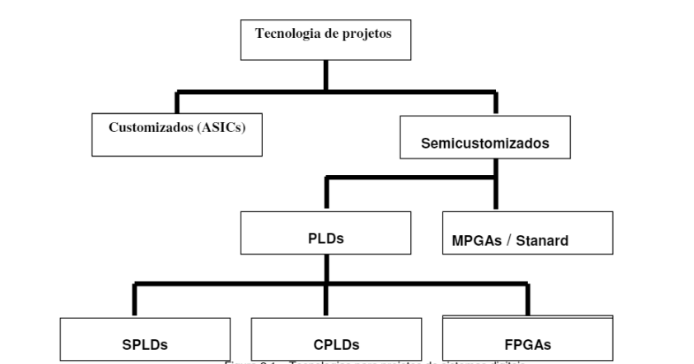
\includegraphics[width=0.7\textwidth]{figuras/Figura1.png}
	 \vspace{-0.2cm}
	\\\textbf{\footnotesize Fonte: \citeonline{Freitas2015} }
	\label{fig:figura1}
\end{figure}
\vspace{-0.5cm}

   \newpage
   
\subsubsection{\esp ASICs (Application-Specific Integrated Circuit ou IC)}

ASISCs ou também conhecidos como IC envolve um alto custo de fabricação, principalmente devido a sua necessidade de uma fabricação especial a depender de cada projeto, apesar de que em projetos de grande escalas esse custo tende a ser amortizado.

\begin{citacaodireta}
Os circuitos integrados digitais implementados em pastilha de silício podem ser classificados como circuitos digitais padrão ou circuitos digitais de aplicações específicas ASICs (Aplication Specific Integrated Circuits). Os circuitos padrões são constituídos por portas lógicas (AND,OR,NOT e Flip – Flops) e necessitam de vários componentes externos para a realização de uma função específica. Os circuitos integrados ASICs são aqueles que precisam de um processo de fabricação especial, que requer máscaras específicas para cada projeto. Outra característica dos circuitos integrados ASICs é o tempo de desenvolvimento longo e os custos extremamente altos. Geralmente não necessitam de muitos componentes externos para a realização de uma função específica, pois sua alta densidade os torna aptos para a implementação de vários tipos de aplicação. Em ambos os casos, os circuitos integrados digitais possuem suas funções internas predefinidas, implementadas na sua construção no processo de fabricação
\cite[25]{Oliveira2011}.
\end{citacaodireta}


\subsubsection{\esp SPLD (Simple Programmable Logic Device):}

Os SPLD se caracterizam por serem dispositivos lógicos programáveis simples, no entanto com menor capacidade lógica em comparação com aos CPLDs e FPGAs, sendo aplicáveis apenas em circuitos lógicos básicos, tendo também como benefício a capacidade de serem reconfiguráveis o que permite modificações durante o desenvolvimento de projetos e consequentemente uma redução dos custos quando se comparado a projetos feitos com outras tecnologias
\cite{Freitas2015}

\begin{citacaodireta}
Segundo a Universidade de São Paulo (2021), "os SPLDs são frequentemente compostos por estruturas como portas lógicas programáveis (AND, OR, NOT) e flip-flops, e têm sido amplamente usados para realizar funções lógicas simples em sistemas embarcados. Esses dispositivos estão se tornando obsoletos devido ao surgimento de tecnologias mais avançadas, como os CPLDs e FPGAs, que oferecem maior flexibilidade e capacidade de integração".
\cite[25]{USP-eDisciplinas}.
\end{citacaodireta}

\subsubsection{\esp SOC (System on Chip)}

Caracterizado por “combinar” todos os componentes de um sistema eletrônico em um único chip, como CPU, memória, interface de entrada/saída, entre outros periféricos. Devido a uma alta integração e eficiência energética se torna uma ótima opção para dispositivos móveis e eletrônicos  

\subsubsection{\esp FPGA  (Field Programmable Gate Array)}

Diferentemente dos ASISCs os FPGAs possuem como características principais a flexibilidade e capacidade de prototipagem rápida, possuindo em sua estrutura milhões de blocos lógicos configuráveis, ideias para sistemas que exigem modificações frequentes principalmente em aplicações de computação acelerada, como processamento de sinais. \cite{Rao2023}

\begin{citacaodireta}
Segundo a Universidade de São Paulo (2021), "os SPLDs são frequentemente compostos por estruturas como portas lógicas programáveis (AND, OR, NOT) e flip-flops, e têm sido amplamente usados para realizar funções lógicas simples em sistemas embarcados. Esses dispositivos estão se tornando obsoletos devido ao surgimento de tecnologias mais avançadas, como os CPLDs e FPGAs, que oferecem maior flexibilidade e capacidade de integração".
\cite[25]{Rao2023}.
\end{citacaodireta}

\section{\esp Evolução dos Dispositivos Lógicos Programáveis}

\subsection{\esp Os Primeiros Dispositivos lógicos Programáveis}

\subsubsection{\esp PROM (Programmable read-only memory)}

Os PROMs se caracterizam por trazer consigo a possibilidade de ser programável pelo usuário, podendo criar uma customização de circuitos lógicos. Nesse contexto, as linhas de endereço serviam como entradas, enquanto as linhas de dados funcionavam como saídas. Além disso, as funções lógicas geralmente não exigem mais do que alguns termos de produto, e cada PROM inclui um decodificador que gerencia seus endereços de entrada. Contudo, as PROMs revelaram-se como uma solução ineficiente para a implementação de circuitos lógicos e são raramente utilizadas atualmente
\cite{Aragao1998}

\subsubsection{\esp PAL (Programmable Array Logic)}

Buscando superar as deficiências nos PLAs os PAL trouxeram consigo tecnologias de apenas um único nível de programação, e com isso baixos custos e melhor desempenho. Sua arquitetura envolve um plano de portas AND programáveis, que plano OR fixo, abaixo se encontra uma uma figura de um exemplo simplificado de uma PAL retirada do artigo “O CPLD (Dispositivo Complexo de Lógica Programação aplicado em automação industrial)” feito por Tiago Freitas, Thiago Pasqualinoto e Juliano Leão
\cite{Freitas2015}

% Figura
\begin{figure}[ht]
	\centering	
	\caption{Esquema simplificado de um PAL}
	\vspace{-0.4cm}
	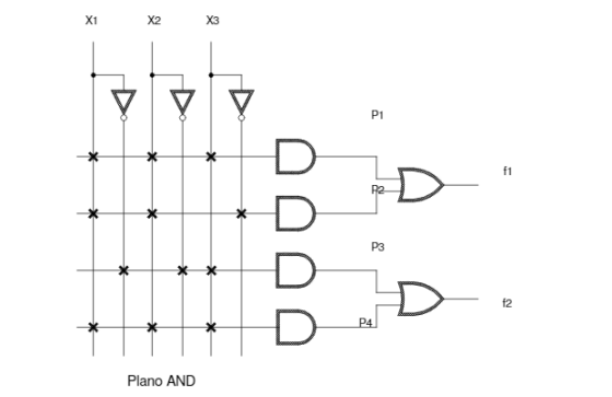
\includegraphics[width=0.7\textwidth]{figuras/Figura2.png}
	 \vspace{-0.2cm}
	\\\textbf{\footnotesize Fonte: \citeonline{Freitas2015} }
	\label{fig:figura2}
\end{figure}
\vspace{-0.5cm}

   \newpage

Novamente a abaixo se encontra uma tabela  feita a partir das informações coletadas nos artigos de CPLD produzidos por Freitas, Pasqualinoto e Leão, e do material de arquitetura de computadores disponibilizado pela USP em https://edisciplinas.usp.br, que busca explicar as principais diferenças entre PROM, PLA e PAL,  em conjunto com uma figura retirada do artigo “A Tecnologia FPGA” feito por António Aragão pelo Instituto de Ciências Matemáticas de São Carlo que demonstra parte da arquitetura dos circuitos em questão.

% Figura
\begin{quadro}[H]
	\centering	
	\caption{Diferenças entre PROM, PLA e PAL}
	\vspace{-0.4cm}
	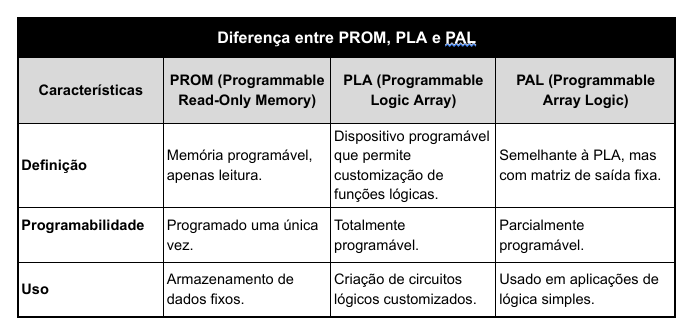
\includegraphics[width=0.7\textwidth]{figuras/Tabela1.png}
	 \vspace{-0.2cm}
	\\\textbf{\footnotesize Fonte: Elaborado pelo autor }
	\label{table: Tabela1}
\end{quadro}
\vspace{-0.5cm}
   
 % Figura
\begin{figure}[H]
	\centering	
	\caption{Esquemas de circuitos de um PROM, PLA e um PAL}
	\vspace{-0.4cm}
	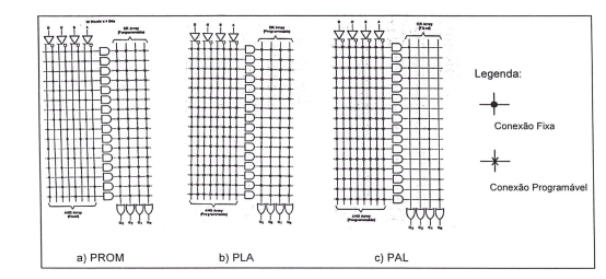
\includegraphics[width=0.7\textwidth]{figuras/Figura3.png}
	 \vspace{-0.2cm}
	\\\textbf{\footnotesize Fonte: \citeonline{Aragao1998} }
	\label{fig:figura3}
\end{figure}
\vspace{-0.5cm}

\section{\esp Principais Diferenças e Características de CPLD e FPGA}

\subsection{ \esp FPGA (Field Programmable Gate Array)}

Devido a seu alto grau de flexibilidade e facilidade de reprogramação, seu uso se destaca em setores elétricos, para processamento digital de sinal como em setores de telecomunicações, principalmente por garantir um alto desempenho em roteadores e switches. Sua arquitetura se baseia em milhões de blocos lógicos configuráveis, denominados CLB (Configuration Logical Block), constituídos praticamente de portas lógicas e flip-flops, tais blocos implementam neste circuito funções lógicas que possibilitam a customização de saídas a partir de determinadas entradas, portanto também podem ser chamados de blocos de entrada e saida (IOB – In/Out Blocks)
\cite{Weber2016}

 % Figura
\begin{figure}[H]
	\centering	
	\caption{Estrutura básica do FPGA}
	\vspace{-0.4cm}
	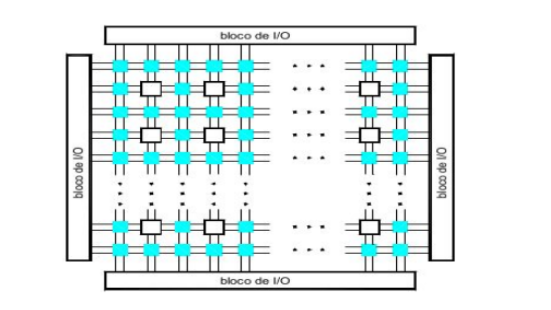
\includegraphics[width=0.7\textwidth]{figuras/Figura4.png}
	 \vspace{-0.2cm}
	\\\textbf{\footnotesize Fonte: \citeonline{Weber2016} }
	\label{fig:figura4}
\end{figure}
\vspace{-0.5cm}

% Figura
\begin{quadro}[H]
	\centering	
	\caption{Possíveis aplicações em FPGAs}
	\vspace{-0.4cm}
	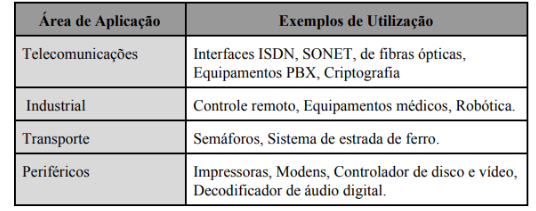
\includegraphics[width=0.7\textwidth]{figuras/Tabela2.png}
	 \vspace{-0.2cm}
	\\\textbf{\footnotesize Fonte: \citeonline{Weber2016} }
	\label{table: Tabela1}
\end{quadro}
\vspace{0.5cm}

\subsection{\esp CPLD (Complex Programmable Logic Device}

Os CPLDs são dispositivos lógicos programáveis menos complexos que os FPGAs, ou seja, com menos flip flops e portas lógicas, sua arquitetura envolve circuitos integrados compostos por portas AND e OR e um banco de macrocélulas. Possuindo também um desempenho mais baixo se comparados com FPGAs, no entanto com algumas vantagens como baixo consumo de energia e melhores tempos de respostas, o que os tornam ideais a sistemas de dispositivos móveis como celulares
\cite{Weber2016}

\vspace{-0.2cm}
 % Figura
\begin{figure}[ht]
	\centering	
	\caption{Representação genérica da arquitetura CPLD}
	\vspace{-0.4cm}
	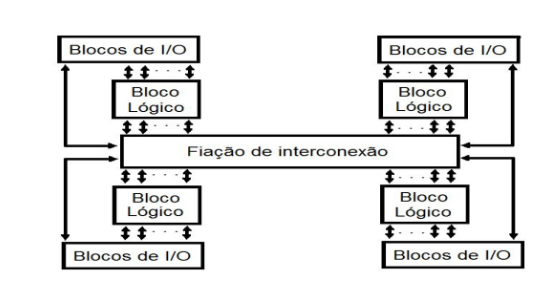
\includegraphics[width=0.7\textwidth]{figuras/Figura5.png}
	 \vspace{-0.2cm}
	\\\textbf{\footnotesize Fonte: \citeonline{Weber2016} }
	\label{fig:figura5}
\end{figure}
\vspace{-0.5cm}

\subsection{\esp Comparação entre arquiteturas CPLD e FPGA}

Abaixo se encontra uma tabela que busca demonstrar as principais diferenças entre circuitos CPLD e FPGA, feita a partir de informações retiradas dos  artigos de CPLD produzidos por Freitas, Pasqualinoto e Leão, “A Tecnologia FPGA”  feito por António Aragão e Eduardo Marques pelo Instituto de Ciências Matemáticas de São Carlo, do artigo “Arquitetura FPGAs e CPLDs da ALTERA” produzido por André Weber, Helenluciany Cechinel, Maria Theisges, e Marcos Moecke”, e do material “CPLD vs FPGA: Differences between them and which one to use?” disponibilizado por Nonato Lab em https://numato.com/kb/cpld-vs-fpga-differences-one-use/.

% Quadro

\begin{quadro}[H]
	\centering	
	\caption{Diferenças entre CPLD e FPGA}
	\vspace{-0.4cm}
	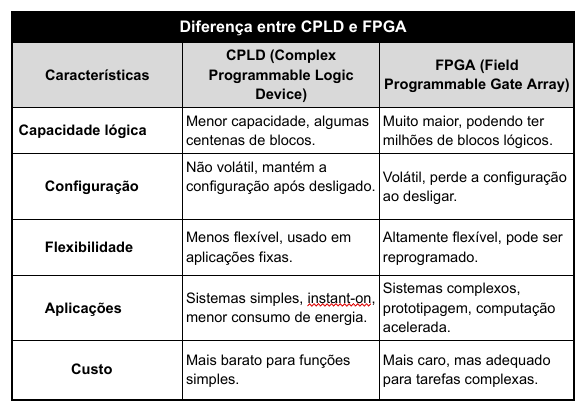
\includegraphics[width=0.7\textwidth]{figuras/Tabela3.png}
	 \vspace{-0.2cm}
	\\\textbf{\footnotesize Fonte: Elaborado pelo autor }
	\label{table: Tabela3}
\end{quadro}
\vspace{-0.5cm}

\section{\esp Conclusão}

O estudo dos Dispositivos Lógicos Programáveis (PLDs), revela-se fundamental para a compreensão das práticas modernas em automação industrial e na arquitetura de computadores. Através da análise de circuitos lógicos e suas aplicações, conseguimos identificar a importância de tecnologias que promovem a flexibilidade, eficiência e escalabilidade em projetos eletrônicos. Oportunizando a construção de uma base teórica mais robusta e uma perspectiva crítica sobre a implementação de soluções em hardware, permitindo o entendimento mais a fundo de projetos de sistemas mais complexos e adaptáveis.




%%%%%%%%%%%%%%%%%%%%%%%%%%%%%%%%%%%
%% FIM DO TEXTO
%%%%%%%%%%%%%%%%%%%%%%%%%%%%%%%%%%%

% \selectlanguage{brazil}
%%%%%%%%%%%%%%%%%%%%%%%%%%%%%%%%%%%
%% Inicio bibliografia
%%%%%%%%%%%%%%%%%%%%%%%%%%%%%%%%%%%

 \newpage
\singlespace{
\renewcommand\refname{REFERÊNCIAS}
\bibliography{bibliografia}
}

%Inclusão do arquivo abntex2-alf.bst como solução para adequação à ABNT NBR 10520:2023 quanto às citações, que não são mais em caixa-alta
\bibliographystyle{abntex2-alf.bst}

\end{document}